\documentclass[tikz, border=10pt]{standalone}
\usepackage{tikz}
\usepackage{amsmath}
\usetikzlibrary{arrows.meta, positioning, fit, backgrounds, calc}

\definecolor{nodeLayerFill}{RGB}{219,234,254}
\definecolor{nodeLayerBorder}{RGB}{37,99,235}
\definecolor{edgeLayerFill}{RGB}{220,252,231}
\definecolor{edgeLayerBorder}{RGB}{22,163,74}
\definecolor{compositeFill}{RGB}{243,244,246}
\definecolor{compositeBorder}{RGB}{75,85,99}
\definecolor{resultFill}{RGB}{254,226,226}
\definecolor{resultBorder}{RGB}{185,28,28}
\definecolor{depFill}{RGB}{254,243,199}
\definecolor{depBorder}{RGB}{180,130,0}

\begin{document}
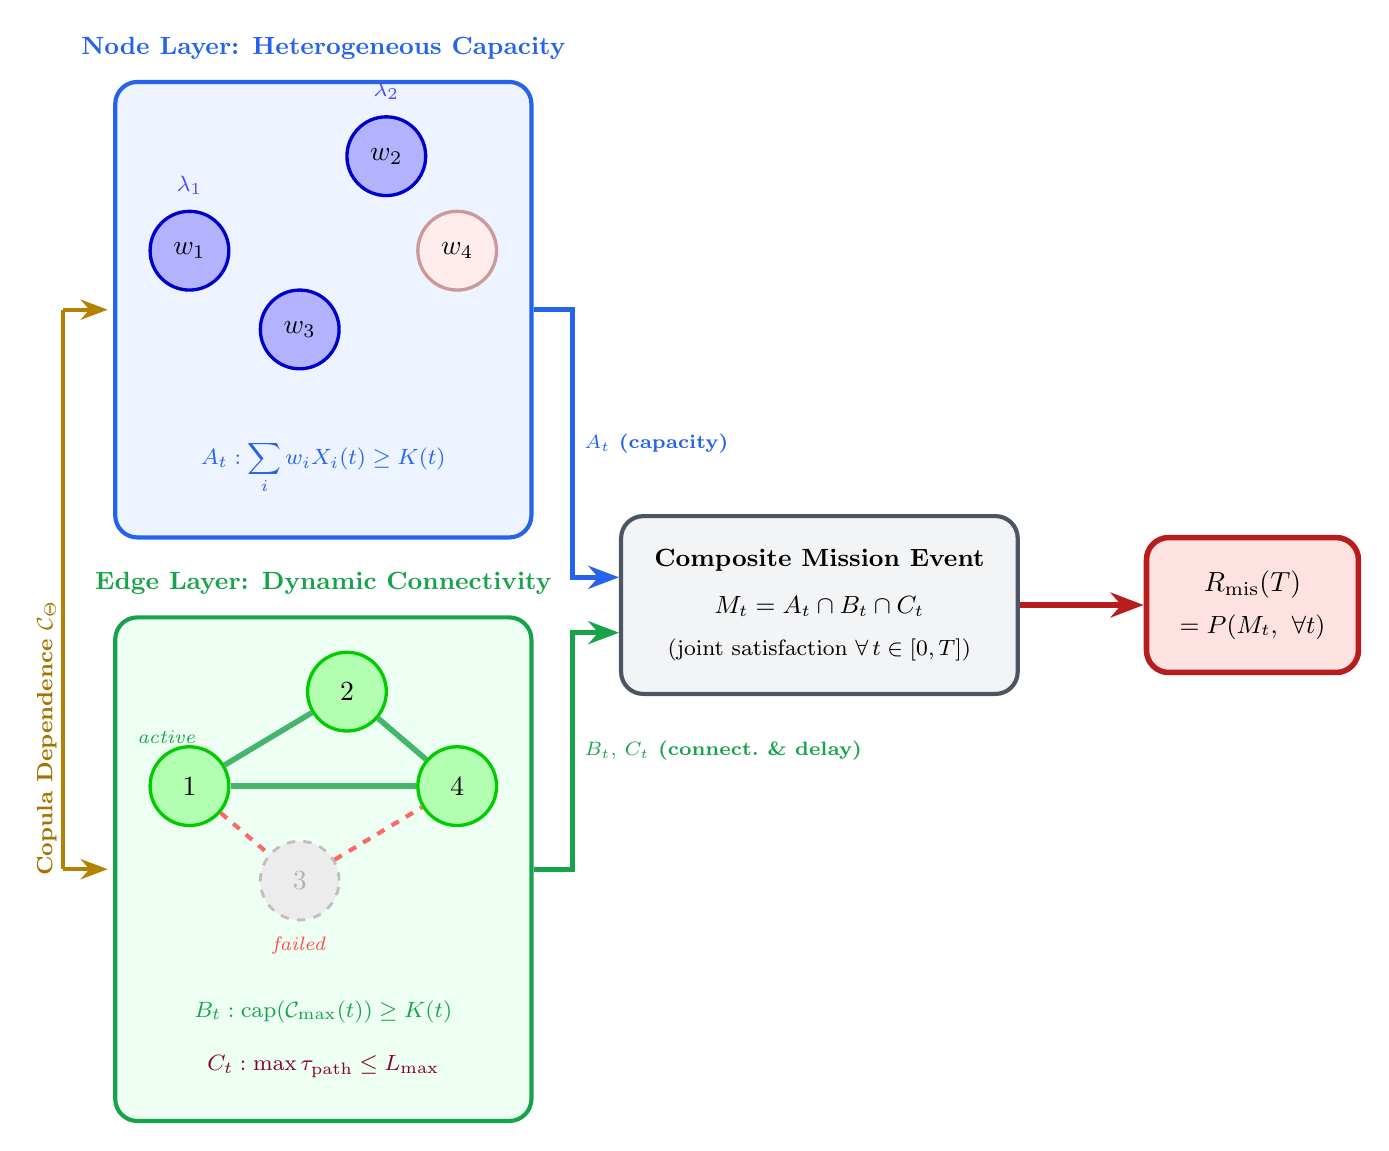
\begin{tikzpicture}[
  % Base font size
  every node/.style={font=\small},
  % UAV node (circle)
  uav/.style={circle, draw=#1!80!black, fill=#1!30, minimum size=1.0cm,
              line width=1.2pt, font=\normalsize\bfseries},
  % Dead node
  dead/.style={circle, draw=gray!50, fill=gray!15, minimum size=1.0cm,
               line width=1pt, dashed, text=gray!60, font=\normalsize},
  % Active communication link
  activeLink/.style={draw=edgeLayerBorder!80, line width=2pt},
  % Failed link
  failedLink/.style={draw=red!60, line width=1.5pt, dashed},
  % Main connector arrow
  mainArrow/.style={-Stealth, line width=1.8pt, color=gray!70},
  % Layer label style
  layerLabel/.style={font=\small\bfseries},
]

%% =====================================================================
%% COLUMN 1 — NODE LAYER (top-left box)
%% =====================================================================

% Agent circles inside the node layer
\node[uav=blue] (n1) at (0, 0)      {$w_1$};
\node[uav=blue] (n2) at (2.5, 1.2)  {$w_2$};
\node[uav=blue] (n3) at (1.4, -1.0) {$w_3$};
\node[uav=pink] (n4) at (3.4, 0)    {$w_4$};

% Failure rate annotations
\node[font=\footnotesize, text=blue!70, above=2pt of n1] {$\lambda_1$};
\node[font=\footnotesize, text=blue!70, above=2pt of n2] {$\lambda_2$};

% Capacity event label at bottom of node layer
\node[font=\footnotesize\bfseries, text=nodeLayerBorder, anchor=north] (capLabel)
  at (1.7, -2.3) {$A_t : \displaystyle\sum_i w_i X_i(t) \geq K(t)$};

% Fit the node layer box
\begin{scope}[on background layer]
  \node[draw=nodeLayerBorder, fill=nodeLayerFill!50, rounded corners=8pt,
        line width=1.5pt,
        fit=(n1)(n2)(n3)(n4)(capLabel),
        inner sep=12pt,
        label={[layerLabel, text=nodeLayerBorder, yshift=4pt]above:%
               \textbf{Node Layer:} Heterogeneous Capacity}
       ] (nodeBox) {};
\end{scope}

%% =====================================================================
%% COLUMN 1 — EDGE LAYER (bottom-left box, below node layer)
%% =====================================================================

% Place edge layer 1.8cm below the node box
\node[uav=green] (e1) at (0,    -6.8) {$1$};
\node[uav=green] (e2) at (2.0,  -5.6) {$2$};
\node[dead]      (e3) at (1.4,  -8.0) {$3$};
\node[uav=green] (e4) at (3.4,  -6.8) {$4$};

% Active links
\draw[activeLink] (e1) -- (e2);
\draw[activeLink] (e2) -- (e4);
\draw[activeLink] (e1) -- (e4);

% Failed links
\draw[failedLink] (e1) -- (e3);
\draw[failedLink] (e3) -- (e4);

% Link annotations
\node[font=\scriptsize, text=edgeLayerBorder, above left=2pt of e1, xshift=18pt]
  {\textit{active}};
\node[font=\scriptsize, text=red!70, below=2pt of e3] {\textit{failed}};

% Connectivity & delay labels
\node[font=\footnotesize\bfseries, text=edgeLayerBorder, anchor=north] (connLabel)
  at (1.7, -9.4) {$B_t : \mathrm{cap}\!\left(\mathcal{C}_{\max}(t)\right) \geq K(t)$};
\node[font=\footnotesize\bfseries, text=purple!70!black, anchor=north] (delLabel)
  at (1.7, -10.1) {$C_t : \max \tau_{\mathrm{path}} \leq L_{\max}$};

% Fit the edge layer box
\begin{scope}[on background layer]
  \node[draw=edgeLayerBorder, fill=edgeLayerFill!50, rounded corners=8pt,
        line width=1.5pt,
        fit=(e1)(e2)(e3)(e4)(connLabel)(delLabel),
        inner sep=12pt,
        label={[layerLabel, text=edgeLayerBorder, yshift=4pt]above:%
               \textbf{Edge Layer:} Dynamic Connectivity}
       ] (edgeBox) {};
\end{scope}

%% =====================================================================
%% COPULA DEPENDENCE — vertical bar on the left with bracket arrows
%% =====================================================================

% Vertical bar connecting midpoints of both layer boxes
\draw[draw=depBorder, line width=1.5pt]
  ([xshift=-18pt]nodeBox.west |- nodeBox.center) --
  ([xshift=-18pt]edgeBox.west |- edgeBox.center)
  node[midway, left=6pt, rotate=90, font=\footnotesize\bfseries,
       text=depBorder!90!black, align=center]
  {Copula Dependence $\mathcal{C}_{\Theta}$};

% Small horizontal ticks to the bars
\draw[draw=depBorder, line width=1.5pt, -Stealth]
  ([xshift=-18pt]nodeBox.west |- nodeBox.center) --
  ([xshift=-2pt]nodeBox.west |- nodeBox.center);
\draw[draw=depBorder, line width=1.5pt, -Stealth]
  ([xshift=-18pt]edgeBox.west |- edgeBox.center) --
  ([xshift=-2pt]edgeBox.west |- edgeBox.center);

%% =====================================================================
%% COLUMN 2 — COMPOSITE MISSION EVENT BOX (centered vertically)
%% =====================================================================

\node[draw=compositeBorder, fill=compositeFill, rounded corners=8pt,
      line width=1.5pt, inner sep=12pt, align=center]
  (composite) at (8.0, -4.5)
  {\textbf{Composite Mission Event}\\[6pt]
   $M_t = A_t \cap B_t \cap C_t$\\[4pt]
   \footnotesize (joint satisfaction $\forall\, t \in [0,T]$)};

%% =====================================================================
%% COLUMN 3 — MISSION RELIABILITY OUTPUT
%% =====================================================================

\node[draw=resultBorder, fill=resultFill, rounded corners=8pt,
      line width=2pt, inner sep=12pt, align=center, font=\normalsize\bfseries]
  (result) at (13.5, -4.5)
  {$R_{\mathrm{mis}}(T)$\\[3pt]
   \small$= P\!\left(M_t,\ \forall t\right)$};

%% =====================================================================
%% ARROWS: layer boxes → composite (angled, clean)
%% =====================================================================

% Node layer → composite
\draw[mainArrow, color=nodeLayerBorder]
  (nodeBox.east) -- ++(0.5, 0) |-
  ([yshift=10pt]composite.west)
  node[pos=0.25, right, font=\scriptsize\bfseries, text=nodeLayerBorder]
  {$A_t$\ (capacity)};

% Edge layer → composite
\draw[mainArrow, color=edgeLayerBorder]
  (edgeBox.east) -- ++(0.5, 0) |-
  ([yshift=-10pt]composite.west)
  node[pos=0.25, right, font=\scriptsize\bfseries, text=edgeLayerBorder]
  {$B_t,\,C_t$\ (connect.\ \& delay)};

% Composite → result
\draw[mainArrow, color=resultBorder, line width=2pt]
  (composite.east) -- (result.west);

\end{tikzpicture}
\end{document}
